%%%%%%%%%%%%%%%%%%%%%%%%%%%%%%%%%%%%%%%%%
% Short Sectioned Assignment
% LaTeX Template
% Version 1.0 (5/5/12)
%
% This template has been downloaded from:
% http://www.LaTeXTemplates.com
%
% Original author:
% Frits Wenneker (http://www.howtotex.com)
%
% License:
% CC BY-NC-SA 3.0 (http://creativecommons.org/licenses/by-nc-sa/3.0/)
%
%%%%%%%%%%%%%%%%%%%%%%%%%%%%%%%%%%%%%%%%%

%----------------------------------------------------------------------------------------
% PACKAGES AND OTHER DOCUMENT CONFIGURATIONS
%----------------------------------------------------------------------------------------

\documentclass[paper=a4, fontsize=11pt]{scrartcl} % A4 paper and 11pt font size

\usepackage[T1]{fontenc} % Use 8-bit encoding that has 256 glyphs
\usepackage{fourier} % Use the Adobe Utopia font for the document - comment this line to return to the LaTeX default
\usepackage[english]{babel} 
\usepackage[utf8]{inputenc}
\usepackage{amsmath,amsfonts,amsthm} % Math packages
\usepackage{tikz} % drawing package

\usepackage{sectsty} % Allows customizing section commands
\allsectionsfont{\centering \normalfont\scshape} % Make all sections centered, the default font and small caps

\usepackage{fancyhdr} % Custom headers and footers
\pagestyle{fancyplain} % Makes all pages in the document conform to the custom headers and footers
\fancyhead{} % No page header - if you want one, create it in the same way as the footers below
\fancyfoot[L]{} % Empty left footer
\fancyfoot[C]{} % Empty center footer
\fancyfoot[R]{\thepage} % Page numbering for right footer
\renewcommand{\headrulewidth}{0pt} % Remove header underlines
\renewcommand{\footrulewidth}{0pt} % Remove footer underlines
\setlength{\headheight}{13.6pt} % Customize the height of the header

\renewcommand{\thesubsection}{\alph{subsection}}

\numberwithin{equation}{section} % Number equations within sections (i.e. 1.1, 1.2, 2.1, 2.2 instead of 1, 2, 3, 4)
\numberwithin{figure}{section} % Number figures within sections (i.e. 1.1, 1.2, 2.1, 2.2 instead of 1, 2, 3, 4)
\numberwithin{table}{section} % Number tables within sections (i.e. 1.1, 1.2, 2.1, 2.2 instead of 1, 2, 3, 4)

\setlength\parindent{0pt} % Removes all indentation from paragraphs - comment this line for an assignment with lots of text

%---- Listings --------------
\usepackage{color}
\definecolor{light-gray}{gray}{0.95}
\usepackage{listings}

\lstnewenvironment{code}[1][]%
{\minipage{\linewidth}
\lstset{ %
language={[x86masm]Assembler},  % choose the language of the code
basicstyle=\footnotesize,       % the size of the fonts that are used for the code
numbers=left,                   % where to put the line-numbers
numberstyle=\footnotesize,      % the size of the fonts that are used for the line-numbers
stepnumber=1,                   % the step between two line-numbers. If it is 1 each line will be numbered
resetmargins=true,              % reset line numbers
numbersep=5pt,                  % how far the line-numbers are from the code
backgroundcolor=\color{white},  % choose the background color. You must add \usepackage{color}
showspaces=false,               % show spaces adding particular underscores
showstringspaces=false,         % underline spaces within strings
showtabs=false,                 % show tabs within strings adding particular underscores
frame=single,                   % adds a frame around the code
tabsize=2,                      % sets default tabsize to 2 spaces
captionpos=b,                   % sets the caption-position to bottom
breaklines=true,                % sets automatic line breaking
breakatwhitespace=false,        % sets if automatic breaks should only happen at whitespace
escapeinside={\%*}{*)},         % if you want to add a comment within your code
morekeywords={
    orr, ldr, bne, subs
    },                          % additional keywords to expand the asm language
#1
}}%
{\endminipage}

%----------------------------------------------------------------------------------------
% TITLE SECTION
%----------------------------------------------------------------------------------------

\newcommand{\horrule}[1]{\rule{\linewidth}{#1}} % Create horizontal rule command with 1 argument of height

\title{
\normalfont \normalsize
\textsc{TDT4205 Compilers, NTNU} \\ [25pt] % Your university, school and/or department name(s)
\horrule{0.5pt} \\[0.4cm] % Thin top horizontal rule
\huge Problem Set 6 \\ % The assignment title
\horrule{2pt} \\[0.5cm] % Thick bottom horizontal rule
}

\author{Stian Jensen} % Your name

\date{\normalsize 27. March 2014} % Today's date or a custom date

\begin{document}

\maketitle % Print the title

%----------------------------------------------------------------------------------------
% PROBLEM 1
%----------------------------------------------------------------------------------------

\section{Optimization}

\subsection{CSE}

Detects repeated subexpressions throughout expressions, and instead calculates them once and store their result in a variable. Storing an extra variable is usually cheaper than calculating the expression multiple times.

No CSE optimizations can be done on the given program.

\subsection{Copy propagation}

Removes instances of direct assignments, i.e. where one value is simply assigned to a variable.
This is done by replacing uses of the variable being assigned to by the value being assigned.

In the given flow graph the line `j = i` could be removed by rewriting `d = j + 2` to `d = i + 2`.

\subsection{Code motion}

Moves code from inside a loop to before the loop, if it is not really necessary for the code to be executed inside. This holds for any expression that isn't dependent (directly or indirectly) on the looping variable(s).
This results in executing the expressions once, instead of once for every iteration of the loop.

In the example we could move the line `t = a * c` and `d = 0` out.

\subsection{Dead code elimination}

Removing code that has no effect on the program execution.

In the example, the assignment `d = 0` can be removed.
It also seems as though the variables e and f have no effect on the program execution, and we may also remove the two lines involving them.

\section{Optimization}

\subsection{Induction variables \& strength reduction}
An induction variable is a variable which increases (or decreases) by a fixed amount in each iteration of a loop. The term is also used for variables which are linearly dependent on an induction variable.

Reduction in strength means replacing a complex expression like multiplication with a simpler one, in this instance addition.
In relation to indirect induction variables this means declaring the variable outside of the loop, and adding the iteration variable to the outer variable once per iteration. This is much simpler of an operation than multiplying a variable by a constant term on each iteration.

\subsection{Flow-graph}

\begin{figure}[ht!]
\centering
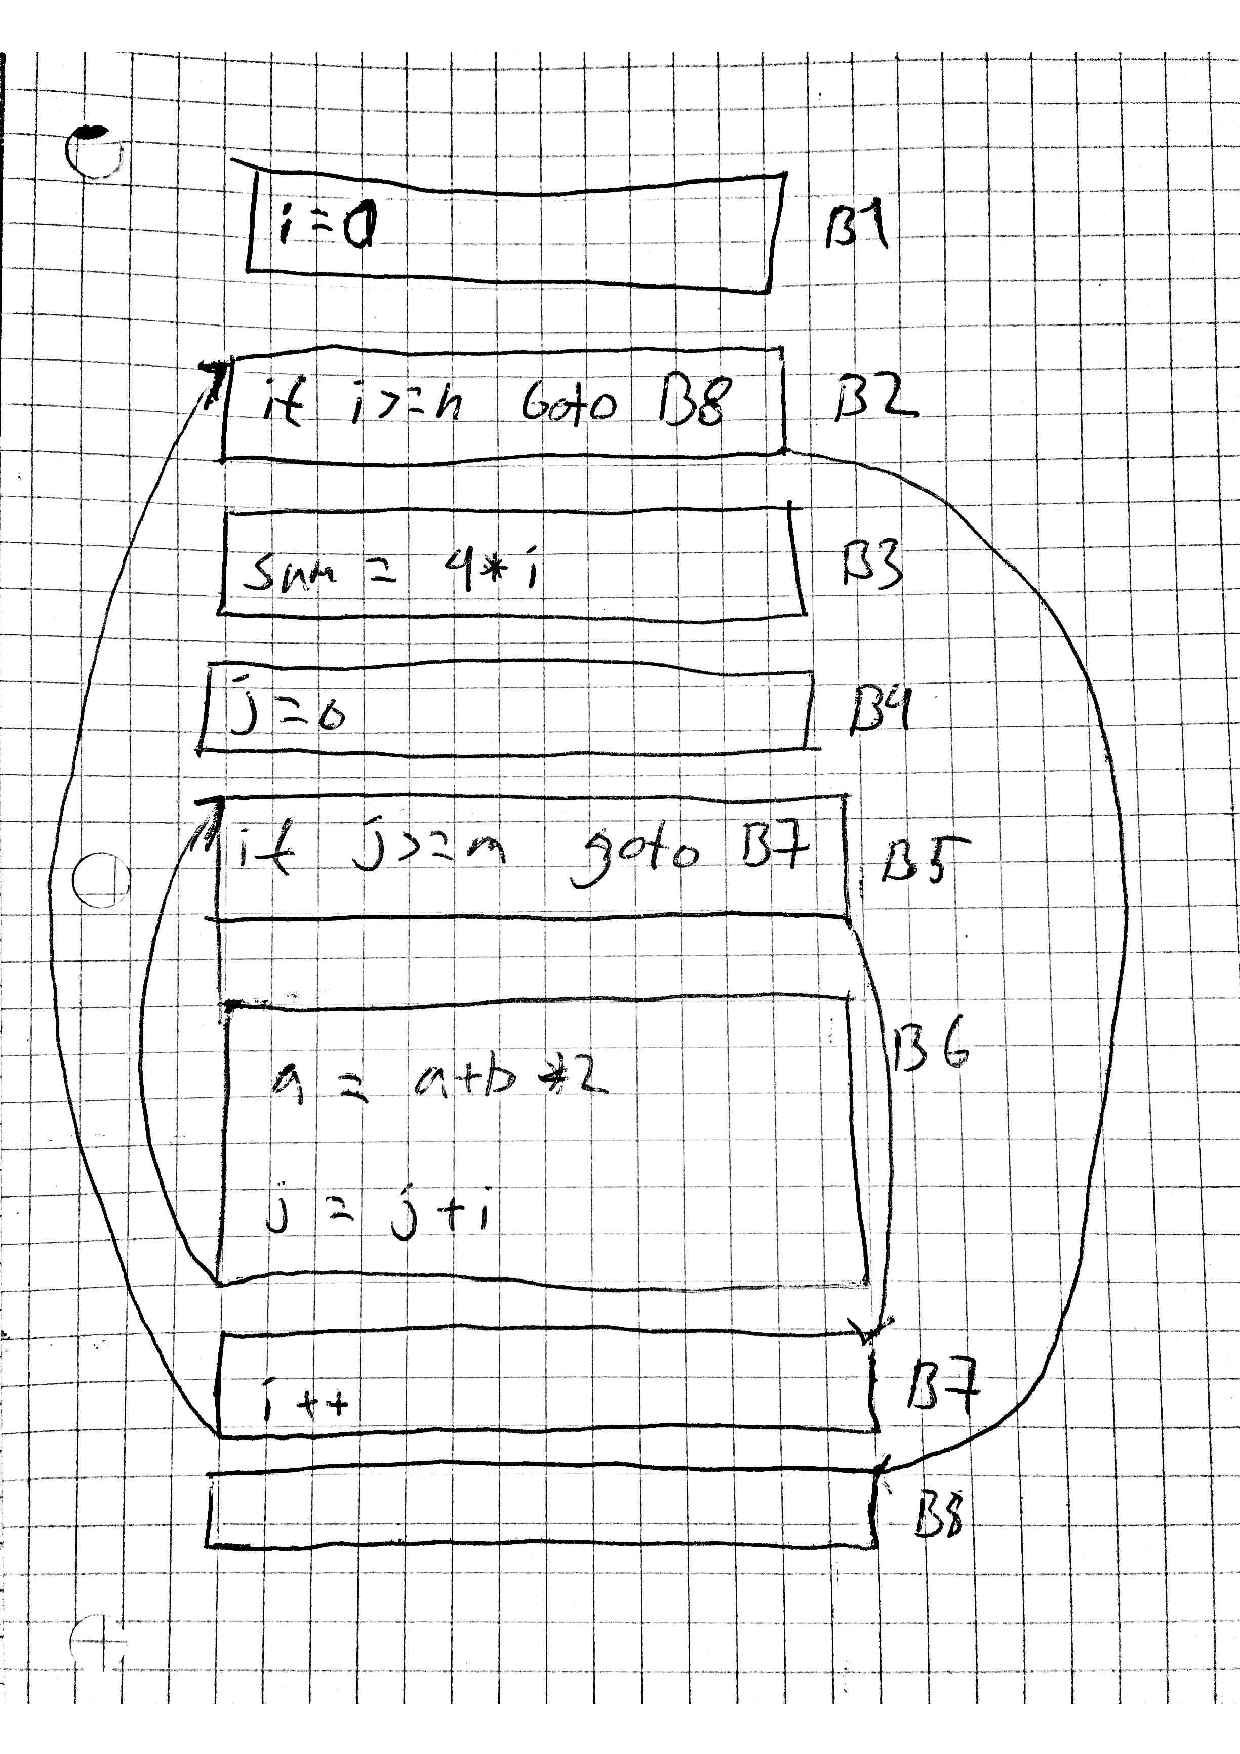
\includegraphics[width=80mm]{2b.pdf}
\end{figure}

\subsection{Optimized flow-graph}

\begin{figure}[ht!]
\centering
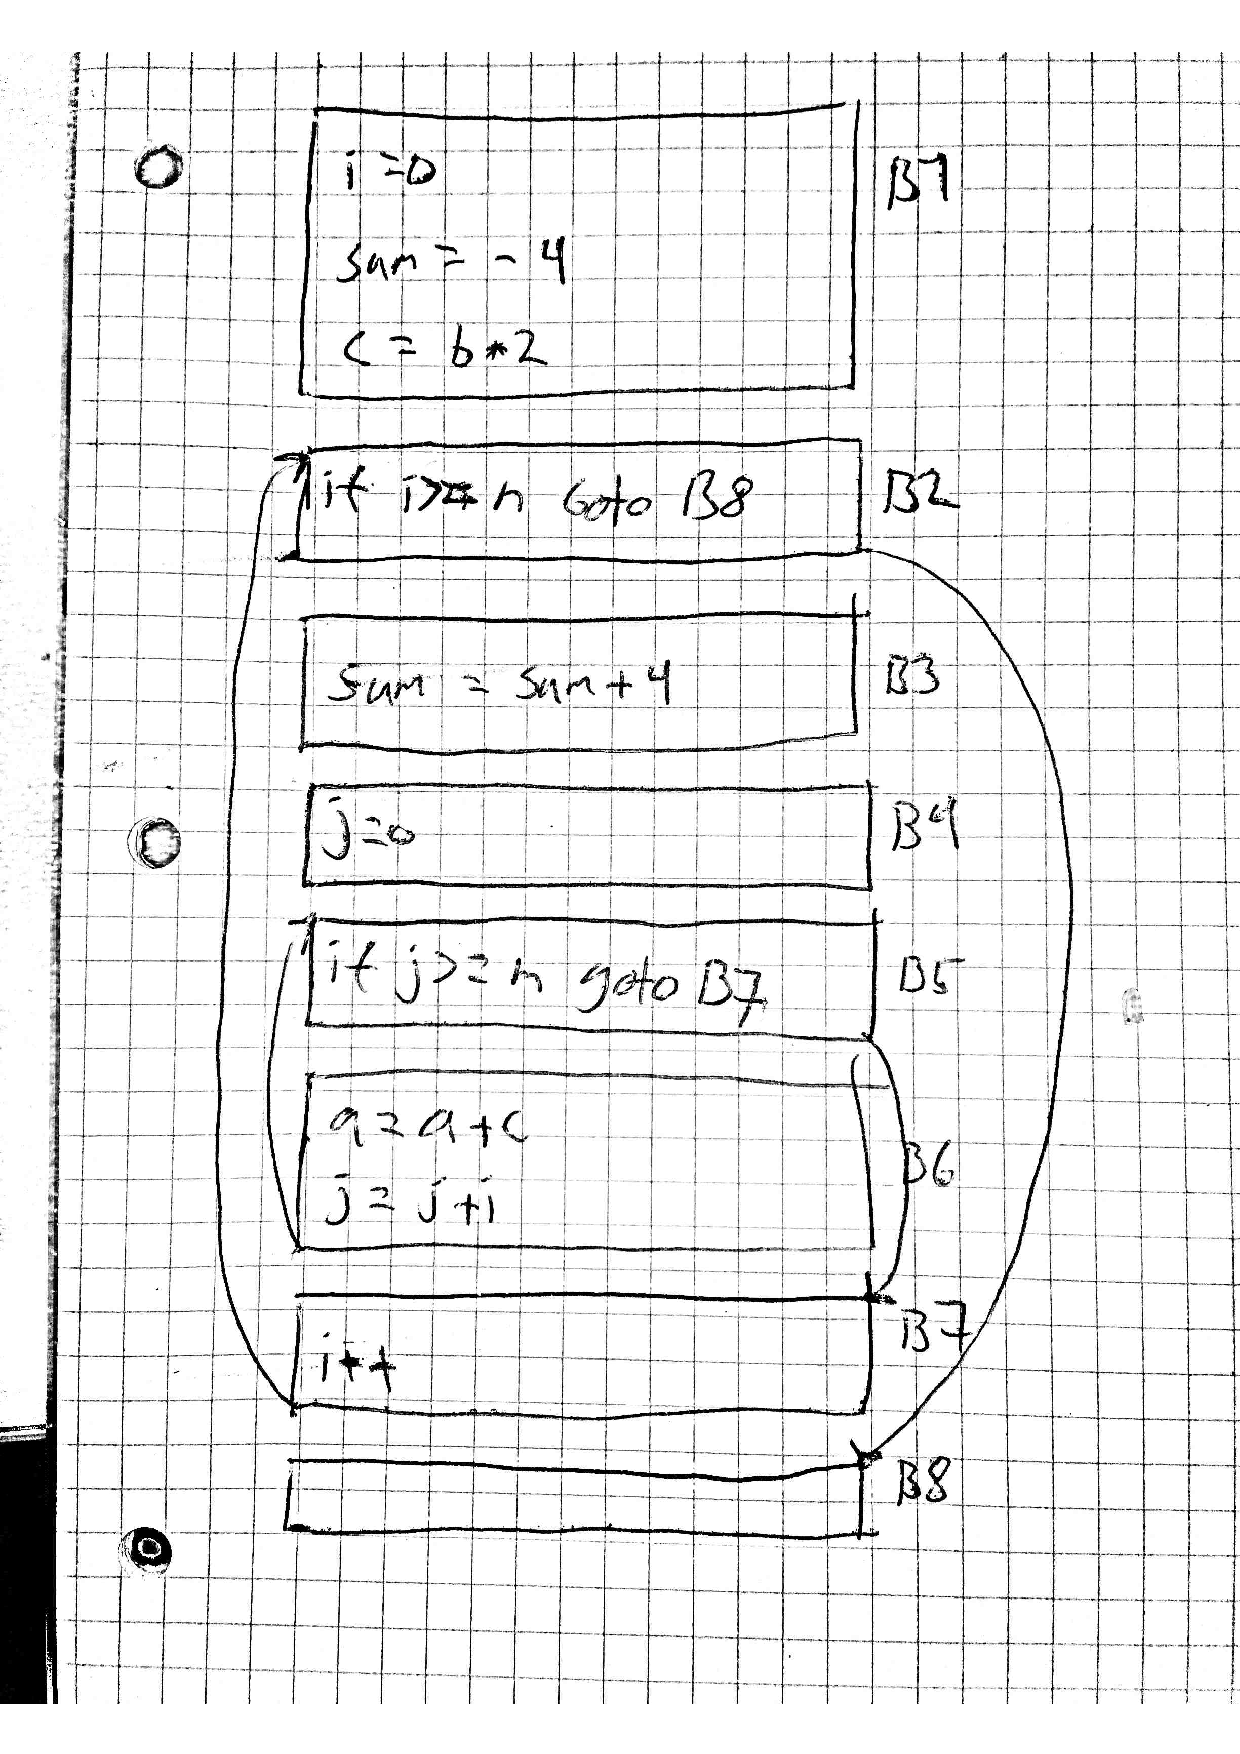
\includegraphics[width=80mm]{2c.pdf}
\end{figure}

\newpage

\section{Data-flow analysis}

\subsection{Reaching definition analysis}

A definition reaches a point in the code if no other definition comes in between and sets a new value for the same variable.

\subsection{Reaching definition data-flow analysis}

\begin{lstlisting}
GEN[1] = {d1, d2, d3}
KILL[1] = {d5, d6, d8, d10, d11, d12}

GEN[2] = {d4, d5}
KILL[2] = {d1, d10}

GEN[3] = {d6, d7}
KILL[3] = {d2, d8}

GEN[4] = {d8, d9}
KILL[4] = {d6, d2}

GEN[5] = {d10, d12}
KILL[5] = {d1, d3, d5, d11}

IN[1] = {}
OUT[1] = {d1, d2, d3}

IN[2] = {d1, d2, d3}
OUT[2] = {d4, d5, d2, d3}

IN[3] = {d4, d5, d2, d3}
OUT[3] = {d6, d7, d3, d4, d5}

IN[4] = {d2, d3, d4, d5}
OUT[4] = {d8, d9, d3, d4, d5}

IN[5] = {d3, d4, d5, d6, d7, d8, d9}
OUT[5] = {d10, d12, d4, d7, d8, d9}
\end{lstlisting}

\subsection{Data-flow analysis}

The IN-set for the exit node equals the out-set from the node B5.
All definitions for the variable b in that set are constant assignment.

\section{Register allocation}

\subsection{Live variables}
A variable is \textbf{live} if it's value may be read in the future.

\subsection{Live variable analysis}

\begin{code}
a = b + c // {b, c}
d = a + b // {a, b, c}
e = 2 * a // {a, c}
a = e + c // {a, c, d, e}
b = d + a // {a, d, e}
c = e - 2 // {e}
\end{code}

\subsection{Register interference graph}

\begin{figure}[ht!]
\centering
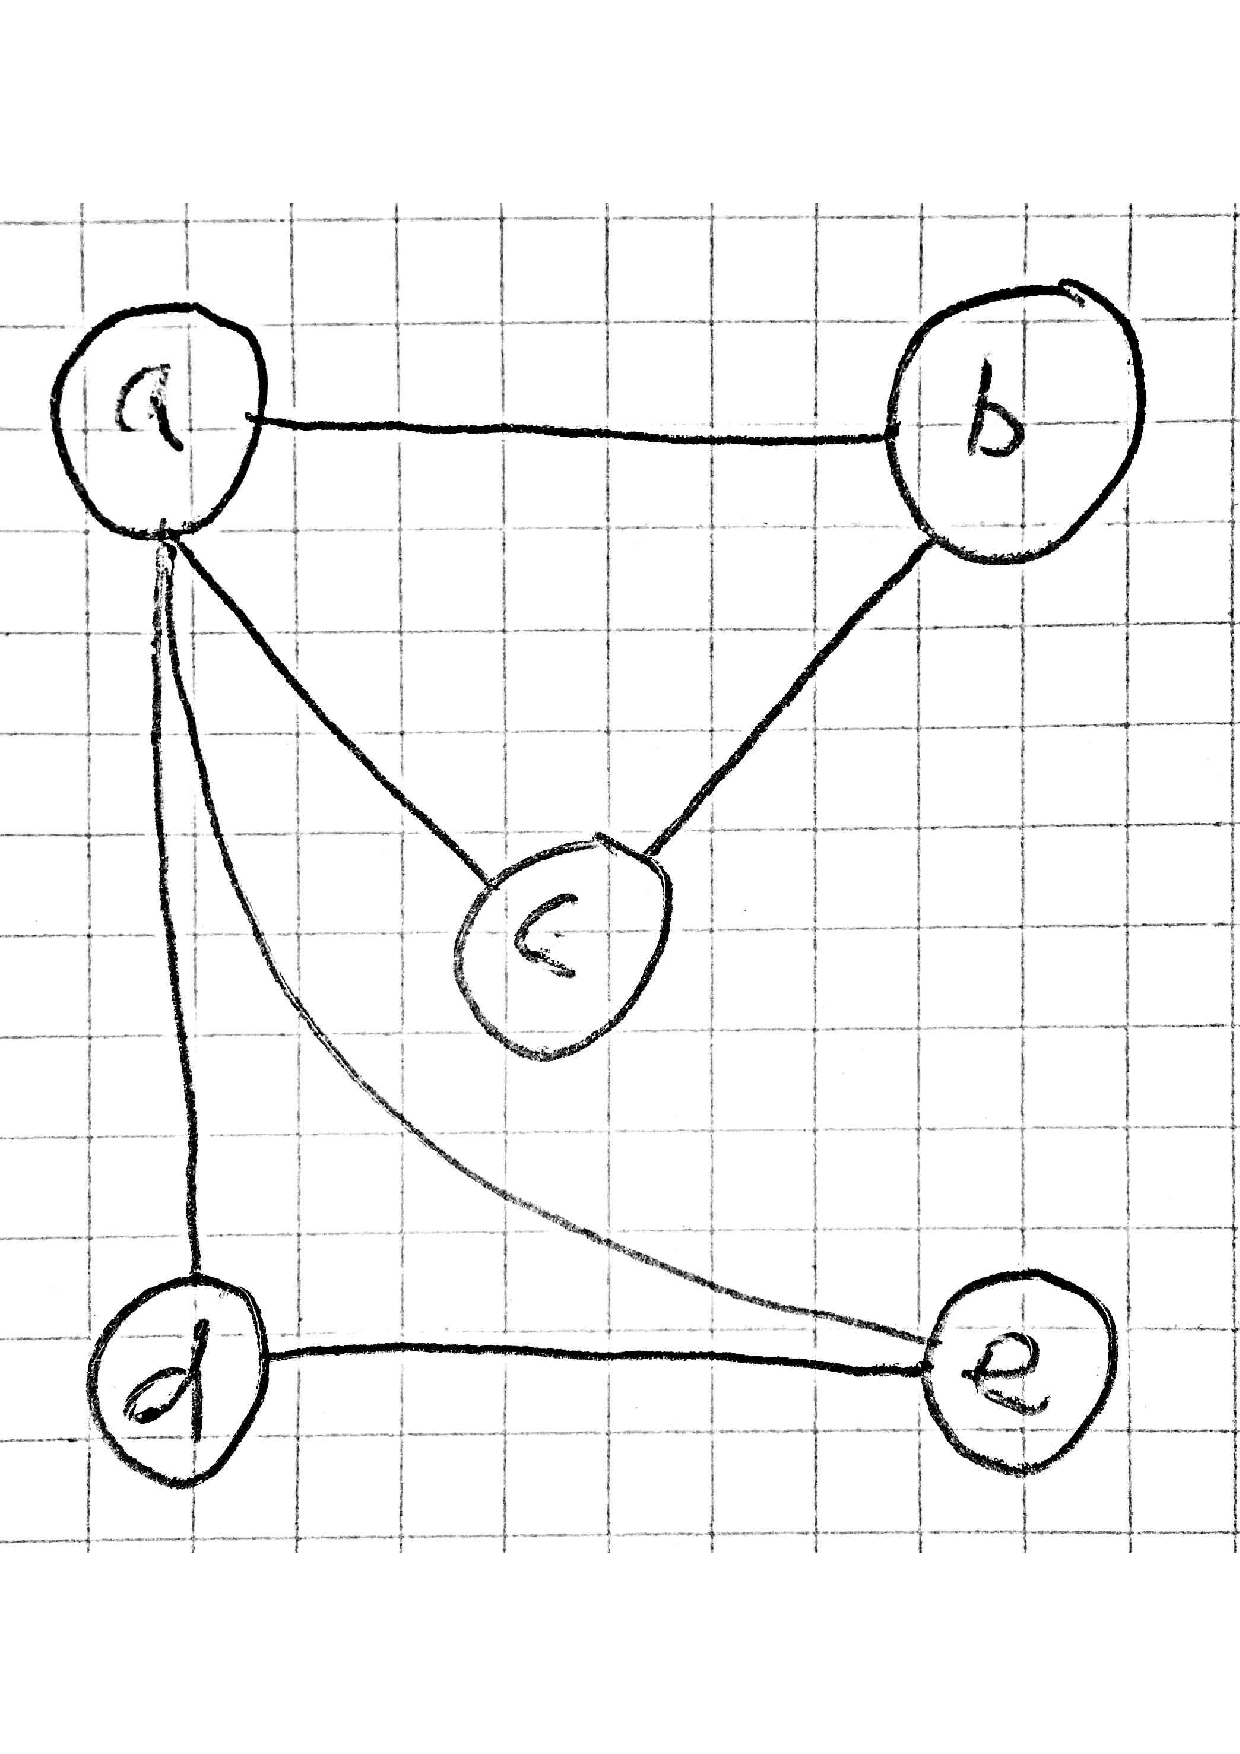
\includegraphics[width=80mm]{4c.pdf}
\end{figure}

\subsection{Register spills}

We will need four registers to avoid spilling. This is because at one point, four variables are live at the same time.

\end{document}
